%++++++++++++++++++++++++++++++++++++++++
% Don't modify this section unless you know what you're doing!
\documentclass[letterpaper,12pt]{article}
\usepackage{tabularx} % extra features for tabular environment
\usepackage{amsmath}  % improve math presentation
\usepackage{graphicx} % takes care of graphic including machinery
\usepackage[margin=1in,letterpaper]{geometry} % decreases margins
\usepackage{cite} % takes care of citations
\usepackage[final]{hyperref} % adds hyper links inside the generated pdf file
\hypersetup{
	colorlinks=true,       % false: boxed links; true: colored links
	linkcolor=blue,        % color of internal links
	citecolor=blue,        % color of links to bibliography
	filecolor=magenta,     % color of file links
	urlcolor=blue         
}
%++++++++++++++++++++++++++++++++++++++++


\begin{document}
	
	\title{COMP 512 Final Project Report}
	\author{Yiwei Xia and Marie Payne}
	\date{\today}
	\maketitle
	
	\pagebreak
	
	\section{Introduction}
	
	The goal of our project is to design and develop a distributed system where clients can make requests and servers deliver responses based upon them, with the use of a middleware server, as well as servers to manage the locking mechanisms and transaction implementation. The aim is to develop this system using the Transmission Control Protocol (TCP), and to make it robust to system failures, and to uphold data integrity through data persistance.
	
	\section{Theory}
	Remote method invocation is defined as one object calling the method of another object potentially located on a remote machine (e.g. usually not local). In RMI architecture, the sender on host A invokes the method B.function(x,y) which is typically the proxy method of the local proxy object (the interface with which A can use to call methods of B). This then gets sent to the RMI layer. The method is packaged into a message (commonly a TCP/UDP packet) to be transmitted over the network to the host machine B. B processes it through the RMI layer and executes the method with the specified parameters (if given), and returns the output to A if it produced any. By using the library java.rmi.Remote, any object that extends it becomes an object that can be used and accessed remotely. The invoker object machine maintains a remote object lookup proxy table, which stores a remote object reference and a real object reference. When the method invocation is transmitted to the server (in this case, host B which is executing the method request from host A, the client), it looks up a the corresponding local object reference that calls the real object. When a remote object reference arrives in a reply message to the client, it looks up the proxy object (interface) to confirm the correct format. \\
	
	The implementation of Remote Method Invocation is to declare the remote interfaces being implemented, so that the remote objects can be called without knowing the implementation ahead of time. A constructor must be defined for the remote object, so that it can be instantiated. The server must contain an implementation of each remote method in the remote object, which is made available to the RMI runtime environment, so that it will be processed through the RMI registry and made available to any potential clients. To call the remote object the hostname of where the object resides must be known, so that its RMIRegistry can be referenced. \\
	
	RMI client-server architecture can be paired with a  middleware server setup to achieve a total distributed information system. The communication middleware server is what any potential client applications communicate with, and all remote method invocations are passed through this server and distributed to the corresponding resource manager server applications to be executed. The middleware server contains some functionality and can process minimal requests to lower overhead costs, however the bulk of the computation is performed on the resource manager servers' side. The following figure demonstrates this architecture, taken from Tanenbaum's Distributed Systems: Principles and Paradigms$.^{[1]}$
	
	\pagebreak
	
	
	\begin{figure}[ht] 
		% read manual to see what [ht] means and for other possible options
		\centering 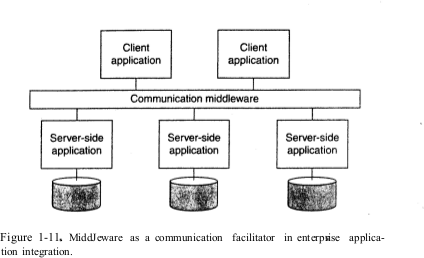
\includegraphics[width=0.8\columnwidth]{figure1.png}
		% note that in above figure file name, "sr_setup",
		% the file extension is missing. LaTeX is smart enough to find
		% apropriate one (i.e. pdf, png, etc.)
		% You can add this extention yourself as it seen below
		% both notations are correct but above has more flexibility
		%\includegraphics[width=1.0\columnwidth]{sr_setup.pdf}
		
	\end{figure}
	
	The Transmission Control Protocol (TCP) is a blocking, connection-oriented, reliable communication protocol which is established on the handshaking protocol and relies on input/output buffers at both ends of the communication channel. The protocol executes based on FIFO delivery principles and acknowledgement packets to provide reliability of the messages being transmitted. The client machine and server machine first transmit handshaking packets to determine that the communication channel is reliable and the hosts are as they declare themselves to be. TCP uses a sequence number on each packet so that they are guaranteed to be transmitted in the correct order, and that the message doesn't be corrupted or duplicated along the network. Acknowledgement packets or acks are sent after every message is received, to confirm transmission (message delivery guarantee). A checksum field is also included in the message to verify the message's contents. The following figure demonstrates the TCP protcol between an example client machine and several servers, processed through a switch (or middleware server)$.^{[1]}$\\
	
	
	In Java, messages can be passed through TCP by using streams of data transmitted over sockets. This also allows objects/methods to be passed over client and server machines, so that objects and methods can be remotely accessed and executed. These streams can be in in XML or JSON, for easy read/write capabilities.
	
	\begin{figure}[ht] 
		% read manual to see what [ht] means and for other possible options
		\centering 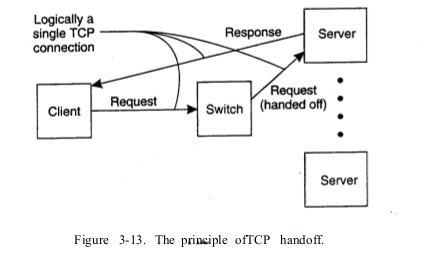
\includegraphics[width=0.8\columnwidth]{figure2.png}
		% note that in above figure file name, "sr_setup",
		% the file extension is missing. LaTeX is smart enough to find
		% apropriate one (i.e. pdf, png, etc.)
		% You can add this extention yourself as it seen below
		% both notations are correct but above has more flexibility
		%\includegraphics[width=1.0\columnwidth]{sr_setup.pdf}
		
	\end{figure} 
	\pagebreak
	
	\section{Design}
	
	We implemented the RMI middleware server by extending the resource manager class, so that the middleware server is technically a fully functioning resource manager server with added functionality. The ports for the RM servers for each resource (car, flight, hotel rooms, customers) are hard-coded. The RM servers are considered and instantiated as clients on the middleware end, and communicated with under that assumption. The RM servers directly trasmit back to the clients. \\
	
	We implemented the TCP middleware server by considering each of the resource manager servers as clients. The middleware, clients, and resource manager servers are run as threads with a hardcoded socket number (the Runner classes). The clients instantiate an input/output stream and connect through the middleware server's thread. The data is passed as JSON to be parsed. Using threads for each connection allows the possibility of multiple clients to use the resources, each with blocking functionality. \\
	
	Our original system consisted of 1 client, 1 middleware, and 4 RMs, one each for flights, cars, hotels, and customers.\\
	
	In our system, implementing locks and transactions required a change to the ResourceManager interface. However, the original inteface was good when used to communicate between the middleware and the RMs. Instead of modifying it and forcing to accomodate functionality it didn't need, a new interface was created called TransactionalResourceManager, which implemented the start, commit, abort functions. Naturally, there is also a new TransactionalMiddleware, which accepts the new start, commit, abort functions.\\
	
	In our system, locking is managed by a LockManager. This manager is different from the provided one in that it doesn't differentiate between timeouts/deadlocks and acquired/redundant locks. When the middleware requests a lock on an object, it simply returns true within the timeout (10 seconds) if the lock has been acquired, or false once that time limit has been reached. This puts the responsibility of detecting deadlocks on the middleware. Client is not aware of locks. Locks are acquired by the middleware automatically as needed for each function call, and released after commit/abort, as per 2PL.\\
	
	Transactions are managed by a TransactionManager. The TransactionManager has a stack of ``requests'' for each transaction, and supports 4 functions, start, commit, abort, and addRequest. The stack of requests keep track of the changes needed to revert the RMs back to their original states in case of an abort. Everytime the middleware performs a modification, i.e. a write, it calls addRequest to and pushes opposite request to the stack for that transaction in the transaction manager. \\
	
	For example, if the client requests createResource(), the transactionalMiddleware will first lock the necessary resource. Then, it will create the resource on the appropriate RM, and then will push a deleteResource() request to the transaction stack in the transaction manager. If the transactionalMiddleware were to fail at this point, and was irrecoverable, the change would have effectively been committed. However, since we're assuming no failures, this is not a problem. Now, if a commit message is sent, the changes are already in the RMs, the transacation manager clears the stack for that transaction, and no more work is needed. However, in the case of a deadlock/abort situation, the transaction will pop every request in the stack, restoring the RMs into their original condition. Because 2 phase locking is used, popping the entire stack is guaranteed to return the RMs to their original conditions.\\
	
	In order to push functions onto stacks, the command pattern was used to create two sets of classes in accordance to the the ResourceManager and TransactionalResourceManager interfaces.\\
	
	With the way aborts work, it was necessary to create ''doubles'' of each function. If the TransactionalMiddleware create() function were to push the TransactionalMiddleware delete() function onto the stack, popping that delete function would push a create() function onto the stack, making an endless loop. Instead, the TransactionalMiddleware create() function pushes the Middleware delete() function onto the stack, whose operations are final (the same way they were implemented in project one).\\
	
	In the third phase of the project, the data persistance was done with SQLite, a serverless variant of SQL-compatible databases. The system data is stored locally in the program execution, and committed to the database upon successful transaction execution. If any of the resource manager servers were to crash, their local copies would perish, but any data successfully committed can be queried. Since database read/writes are costly in time, they are only performed when necessary, such as during commits and, sparingly, during method calls.
	
	\section{Performance Analysis Methods}
	
	The performance analysis we conducted on our system included two parts; the first part involving one client and the average response times of different API methods in the system, the second involving muliple clients and varying loads to analyze the response times. Since we're focusing on response times, we want to avoid deadlocking the system as much as possible, which can be done with multiple clients by only using one method, query, which has no possibility of deadlock even called in concurrence (multiple read locks can be acquired at once, in our implementation). \\
	
	The first part of the performance analysis simulated one customer on a loop. Every iteration of the program would choose a method and call it N times to produce an average, and print the response time on the customer side. Doing this narrows down the time spent at each stage in the method call on average, and can thus be used to figure out the bottleneck of the system and analyze where measures to increase efficiency can be implemented.\\
	
	The second part of the analysis simulates multiple customers in a number of threads, and calls methods selected so as to avoid creating a deadlock in a loop. The load is then varied from 1 to 10 (the threads sleep at a time interval adjusted to reflect this) and the average response time recorded. This is then plotted using matplotlib in Python to illustrate the results (each line is for the number of customers, best-fit). This part of the performance analysis is meant to determine the saturation point of the system, with some level of concurrency. However, this test uses an optimal system with no occurrence of deadlocks, when in reality this system will deadlock somewhat frequently when the number of client threads running increases. 
	
	\section{ Performance Analysis Results}
	The results for phase 1 of the performance analysis testing can be resolved in the following table:
	
	\begin{center}
		\begin{tabular}{ |c|c| } 
			\hline
			Method Call: & Client Side (ms) \\
			\hline
			start & 5.43  \\ 
			commit & 5.48  \\ 
			abort & 5.49  \\ 
			createResource & 10.64  \\ 
			updateResource & 10.22  \\ 
			reserveResource & 7.74  \\ 
			deleteResource & 8.85  \\ 
			queryResource & 5.52  \\ 
			uniqueCustomerId & 5.56  \\ 
			createCustomer & 10.78 \\
			queryCustomer & 11.75 \\ 
			deleteCustomer & 10.60 \\ 
			customerAddReservation & 10.94 \\ 
			customerRemoveReservation & 16.44 \\
			itinerary & 42.20\\
			\hline
		\end{tabular}\\
		Figure 1: Averages of method calls in the system in \\milliseconds, using one client and ideal conditions.
	\end{center}
	The method calls were performed in ideal contexts. The itinerary method was called using two resources chosen at random (this is sufficiently varied for our purposes, however it should be noted that using a larger itinerary will scale the average response time linearly with the resource managers used). Each average was taken by running the method call 100 times and averaging the total time, which ended up being overly cautious and unnecessary but smoothed out any minor discrepancies. Running the loops multiple times revealed a standard deviation of +- 0.30 ms, roughly (more testing could be done at this phase to determine the exact standard devation, though this precision is not necessary in the preliminary development phases of this system).\\
	
	The results for the second phase of the analysis are demonstrated in the figure shown:\\
	\begin{figure}[ht] 
		% read manual to see what [ht] means and for other possible options
		\centering 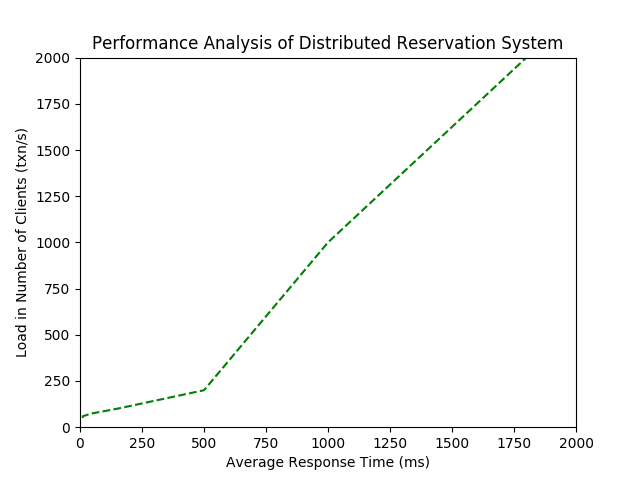
\includegraphics[width=0.8\columnwidth]{performanal.png}
		% note that in above figure file name, "sr_setup",
		% the file extension is missing. LaTeX is smart enough to find
		% apropriate one (i.e. pdf, png, etc.)
		% You can add this extention yourself as it seen below
		% both notations are correct but above has more flexibility
		%\includegraphics[width=1.0\columnwidth]{sr_setup.pdf}
		
	\end{figure}\\
	The only method used in the trials was queryResource, with a lot of instantiated resources that get queried randomly so to prevent the threads from simultaneously accessing the list data structures (this throws a data corruption error). Threads sleep before checking if responses are received, so <10 ms response times are not achievable.
	
	\section{Performance Analysis Discussion}
	For the first part of the performance testing, we used one client on a loop and took the average response time on the client side of each method available in the API. Several of the methods hovered around 10ms or below on average, with the exceptions of customerRemoveReservation and itinerary. These two methods used the most TCP calls compared to the other methods, which were more localized to one resource manager and performed checks against locally stored hashmaps and mutable lists. The performance of itinerary depends on a couple of variables, such as the number of resource managers involved, the number of resource IDs involved, and the size of the mutable map of resources being sent to the middleware server. The testing protocols used randomized two resources equally chosen from the three resource pools, so the reservable item mutable map being passed was a constant size, though the number of resource managers involved could vary. The standard deviation for this method was also larger, but if we accounted for the number of resource managers involved it would scale down to the same margin as the other method calls. More thorough performance testing could be used, but it is likely that the bottleneck of the system is the TCP implementation, specifically the queue the replies are stored in. Since TCP is necessary to operate over a network, this is an acceptable overhead for our purposes.\\
	
	For the second part of the performance analysis testing, it was observed that with a higher number of active clients, the standard deviation varied a lot more (because of the nature of threads, it isn't guaranteed that the method call terminates before switching contexts in runtime, and a higher load made this more volatile). The number of clients is proportional to the amount of load on the system, with an increasing number of clients bringing an increasing load. The response times were steady from 1 to 200 clients and began to exponentially increase around 200. We can conclude that the system remains efficient for loads up to 200 clients, but shows significant strain as the load increases beyond that point.
	
	\section{Conclusion}
	
	The implementation of locking mechanisms through a middleware server promotes concurrency control of the system. Backing up the data to an external source allows data persistance in the system and strengthens the fault tolerance. The bottleneck of the system appears to be the TCP calls sending requests over the network. A more efficient implementation would be to perhaps use a hashmap to store replies in the TCP queues, instead of unneccessarily iterating over all the elements. This system is strong against server crashes at various points in the execution, and is robust against a variety of fault scenarios.
	
	\section{Statement of Contribution}
	Yiwei did the code implementation, the translation into Kotlin, and the testing/error handling for all three phases. Marie did the slides, the reports, the testing, the performance analysis, and the client-side interface. The breakdown was roughly 80-20. 
	
	\section{Bibliography}
	
	All the theory in this report came directly from the lecture slides on the course website or the recommended textbook, Distributed Systems: Principles and Paradigms by Andrew S. Tanenbaum and Maarten Van Steen, Second Edition, Pearson and Prentice Hall, Amsterdam, 2007. 
	
\end{document}
